\documentclass{article}
\title{Fizyka}
\date{2025-02-12}
\author{Bartosz Świst}

\usepackage[utf8]{inputenc}
\usepackage[T1]{fontenc}
\usepackage{amsmath, amssymb, tikz}

\numberwithin{equation}{section}
\DeclareMathOperator{\tg}{tg}
\newcommand{\unit}[1]{\,\left[\mathrm{#1}\right]}

\begin{document}
  \maketitle
  \newpage
  \section{Kinematyka}
    \subsection{Wektory}
      \subsubsection{Iloczyn skalarny}
        \begin{gather}
          c = \vec a \cdot \vec b\\
          c = |\vec a|\cdot |\vec b|\cdot\cos\measuredangle(\vec a, \vec b)
        \end{gather}
      \subsubsection{Iloczyn wektorowy}
        \begin{gather}
          \vec c = \vec a \times \vec b\\
          \vec c = |\vec a|\cdot |\vec b|\cdot\sin\measuredangle(\vec a, \vec b)
        \end{gather}
    \subsection{Opis ruchu}
      \begin{equation}
        v_{\acute sr} = \frac st \unit{\frac ms}
      \end{equation}
      \begin{equation}
        \vec v_{\acute sr} = \frac{\Delta\vec x}{\Delta t} \unit{\frac ms}
      \end{equation}
      \begin{equation}
        \vec a = \frac{\Delta\vec v}{\Delta t} \unit{\frac{m}{s^2}}
      \end{equation}
    \subsection{Ruch jednostajny prostoliniowy}
      \begin{equation}
        v = const.
      \end{equation}
      \begin{equation}
        s = vt
      \end{equation}
      \begin{equation}
        \tg\alpha = \frac st = v
      \end{equation}
      \begin{equation}
        x(t) = x_0 \pm vt
      \end{equation}
    \subsection{Ruch jednostajnie przyśpieszony}
      \begin{gather}
        a = \frac{\Delta v}{\Delta t} \unit{\frac{m}{s^2}}\\
        a = const.
      \end{gather}
      jeżeli $v_0 = 0$:
      \begin{gather}
        v = at\\
        s = \frac{at^2}{2}
      \end{gather}
      jeżeli $v_0 \ne 0$:
      \begin{gather}
        v_k = v_0 + at\\
        s = v_0t + \frac{at^2}{2}
      \end{gather}
      \begin{equation}
        s_1:s_2:s_3:s_4:s_5:\cdots = 1:3:5:7:9:\cdots
      \end{equation}
    \subsection{Ruch jednostajnie opóźniony}
      jeżeli $v_k = 0$:
      \begin{gather}
        v_0 = at\\
        s = \frac{1}{2}v_0t
      \end{gather}
      jeżeli $v_k \ne 0$:
      \begin{gather}
        v_k = v_0 - at\\
        s = v_0t - \frac{at^2}{2} = v_0t - \frac{1}{2}\Delta vt
      \end{gather}
    \subsection{Rzut pionowy}
      \subsubsection{Wznoszenie się}
        \begin{gather}
          h = v_0t - \frac{gt^2}{2}\\
          v = v_0 - gt
        \end{gather}
      \subsubsection{Opadanie}
        \begin{gather}
          h = v_0t + \frac{gt^2}{2}\\
          v = v_0 + gt
        \end{gather}
        jeżeli $v_0 = 0$:
        \begin{equation}
          v = gt
        \end{equation}
    \subsection{Rzut poziomy}
      \begin{gather}
        h = \frac{gt^2}{2}\\
        x = v_0t = v_0\sqrt{\frac{2h}{g}}\\
        v = \sqrt{v_0^2 + v_y^2} = \sqrt{v_0^2 + (gt)^2}
      \end{gather}
    \subsection{Rzut ukośny}
      \begin{center}
        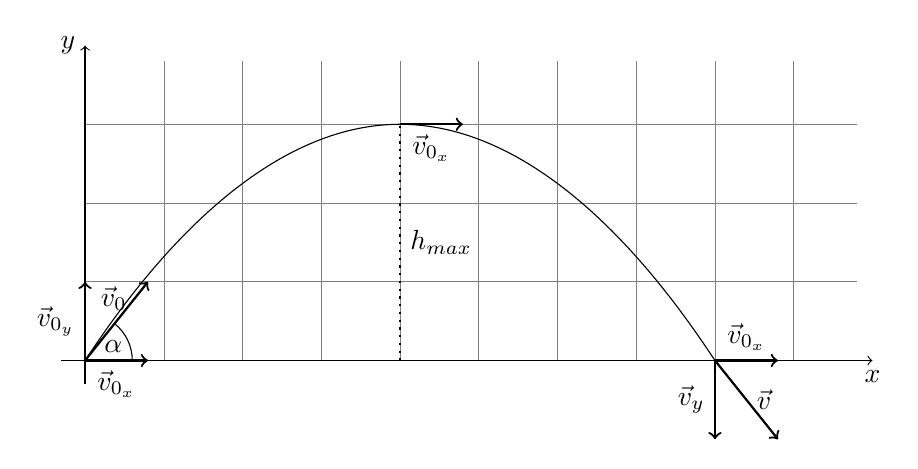
\begin{tikzpicture}
          \draw[gray, very thin] (0, 0) grid (9.8, 3.8);
          \draw[->, thin] (-0.3, 0) -- (10, 0) node[below] {$x$};
          \draw[->, thin] (0, -0.3) -- (0, 4) node[left] {$y$};
          \draw (4, 3) parabola (0, 0);
          \draw (4, 3) parabola (8, 0);

          \draw[->, thick] (0, 0) -- (0.8, 0) node[midway, below] {$\vec v_{0_x}$};
          \draw[->, thick] (0, 0) -- (0, 1) node[midway, left] {$\vec v_{0_y}$};
          \draw[->, thick] (0, 0) -- (0.8, 1) node[midway, above, xshift=-1] {$\vec v_0$};
          \draw (0.6, 0) arc (0:50:0.6) node[below, xshift=-0.8, yshift=-2.5] {$\alpha$};

          \draw[->, thick] (4, 3) -- (4.8, 3) node[midway, below] {$\vec v_{0_x}$};

          \draw[->, thick] (8, 0) -- (8.8, 0) node[midway, above] {$\vec v_{0_x}$};
          \draw[->, thick] (8, 0) -- (8, -1) node[midway, left] {$\vec v_y$};
          \draw[->, thick] (8, 0) -- (8.8, -1) node[midway, right] {$\vec v$};

          \draw[dotted, thick] (4, 0) -- (4, 3) node[midway, right] {$h_{max}$};
        \end{tikzpicture}
      \end{center}
      \begin{align}
        v_{0_x} &= v_0\cos\alpha\\
        v_{0_y} &= v_0\sin\alpha
      \end{align}
      \begin{equation}
        y(x) = x\tg\alpha - x^2\cdot \frac{g}{2v_0^2\cos^2\alpha}
      \end{equation}
      \begin{gather}
        t_c = \frac{2v_0\sin\alpha}{g}\\
        h_{max} = \frac{v_0^2\sin^2\alpha}{2g}\\
        z = \frac{v_0^2\sin 2\alpha}{g}
      \end{gather}
      dla $\alpha = 45^\circ,\; z = z_{max}$:
      \begin{equation}
        z_{max} = \frac{v_0^2}{2g}
      \end{equation}
    \subsection{Ruch jednostajny po okręgu}
      \begin{equation}
        \alpha = \frac Lr \unit{rad}
      \end{equation}
      \begin{gather}
        f = \frac nt \unit{Hz}\\
        \omega = \frac{\Delta\alpha}{\Delta t} \unit{\frac{rad}{s}}
      \end{gather}
      dla jednego obrotu:
      \begin{gather}
        f = \frac 1T\\
        \omega = \frac{2\pi}{T}
      \end{gather}
      \begin{gather}
        v = \frac{2\pi r}{T} = 2\pi rf = \omega r\\
        a_r = \frac{v^2}{r}
      \end{gather}
      \begin{gather}
        \vec v = \vec\omega \times \vec r\\
        v = \omega r\sin\measuredangle(\vec\omega, \vec r)
      \end{gather}
      dla $\vec\omega \perp \vec r$:
      \begin{equation}
        v = \omega r
      \end{equation}
    \subsection{przyśpieszenie w ruchu po okręgu}
      \begin{gather}
        \vec a_s = \frac{\Delta\vec v}{\Delta t}\\
        a_w = \sqrt{a_r^2 + a_s^2}
      \end{gather}

  \newpage
  \section{Dynamika}
    \subsection{Zasady dynamiki Newtona}
      \subsubsection{Pierwsza zasada}
        \begin{equation}
          \vec F_w = 0 \Rightarrow \vec v = 0 \lor \vec v = const.
        \end{equation}
      \subsubsection{Druga zasada}
        \begin{gather}
          F_w \ne 0 \Rightarrow a = const.\\
          \vec a = \frac{\vec F_w}{m} \Rightarrow \vec F_w = m\vec a \unit{N}
        \end{gather}
      \subsubsection{Trzecia zasada}
        \begin{align}
          \vec F_{AB} &= -\vec F_{BA}\\
          F_{AB} &= F_{BA}
        \end{align}
    \subsection{Ruch na równi pochyłej}
      \begin{align}
        \frac{\vec F_Z}{\vec F_g} = \sin\alpha &\Rightarrow \vec F_Z = \vec F_g\sin\alpha = mg\sin\alpha\\
        \frac{\vec F_N}{\vec F_g} = \cos\alpha &\Rightarrow \vec F_N = \vec F_g\cos\alpha = mg\cos\alpha
      \end{align}
    \subsection{tbd}
    \subsection{Pęd ciała}
      \begin{equation}
        \vec p = m\vec v \unit{\frac{kg\cdot m}{s}}
      \end{equation}
      \begin{equation}
        \Delta p = F\Delta t
      \end{equation}
      \subsubsection{Zasada zachowania pędu}
        \begin{equation}
          \Delta \vec p = 0 \Leftrightarrow \vec p = const.
        \end{equation}
      \subsection{Środek masy}
        \begin{equation}
          x_c = \frac{m_1x_1+m_2x_2+\cdots+m_nx_n}{m_1+m_2+\cdots+m_n} =
          \frac{\sum\limits_{i=1}^n m_ix_i}{\sum\limits_{i=1}^n m_i}
        \end{equation}
      \subsection{Tarcie}
        \begin{align}
          T_s &= \mu_sF_N \unit{N}\\
          T_k &\leqslant \mu_kF_N \unit{N}
        \end{align}
      \subsection{Siła dośrodkowa}
        \begin{equation}
          F_{do} = \frac{mv^2}{r} \unit{N}
        \end{equation}
        \subsection{Siła bezwładności}
        \begin{equation}
          \vec F_b = -m\vec a \unit{N}
        \end{equation}

  \newpage
  \section{Praca, moc, energia}
    \subsection{Praca}
      \begin{gather}
        W = \vec F\Delta\vec r \unit{J}\\
        W = F\Delta r \cos\measuredangle(\vec F, \Delta\vec r)
      \end{gather}
      dla $\alpha = 0^\circ$:
      \begin{equation}
        W = F\Delta r = Fs
      \end{equation}
      dla $\alpha = 90^\circ$:
      \begin{equation}
        W = 0
      \end{equation}
    \subsection{Moc}
      \begin{equation}
        P = \frac{W}{t} \unit{W}
      \end{equation}
      dla $v = const.$:
      \begin{equation}
        P = Fs
      \end{equation}
    \subsection{Energia mechaniczna}
      \subsubsection{Energia kinetyczna}
        \begin{align}
          &E_k = \frac{mv^2}{2} \unit{J}\\
          &\Delta E_k = W
        \end{align}
      \subsubsection{Energia potencjalna}
        \begin{align}
          &E_p = mgh \unit{J}\\
          &\Delta E_p = W
        \end{align}
      \subsubsection{Zasada zachowania energii}
        \begin{align}
          &E_c = E_k + E_p\\
          &E_c = const. \Rightarrow \Delta E_c = 0\\
          &\Delta E_c = \Delta E_p + \Delta E_k
        \end{align}
    \subsection{Sprawność}
      \begin{equation}
        \eta = \frac{E_{u\dot{z}yt.}}{E_{pob.}}\: (\cdot 100\%) = \frac{W_{u\dot{z}yt.}}{E_{pob.}}\: (\cdot 100\%)
      \end{equation}
      \begin{equation}
        \eta_{u\dot{z}yt.} = \prod_{i=1}^n \eta_i
      \end{equation}

  \newpage
  \section{Hydrostatyka}
    \subsection{Ciśnienie i parcie}
      \subsubsection{Ciśnienie}
        \begin{equation}
          p = \frac{F_N}{S} \unit{Pa}
        \end{equation}
        dla $F_N = mg$:
        \begin{equation}
          p = \frac{mg}{S}
        \end{equation}
      \subsubsection{Parcie}
        \begin{equation}
          P = pS \unit{N}
        \end{equation}
      \subsubsection{Ciśnienie hydrostatyczne}
        \begin{equation}
          p_h = \frac{P}{S} = \varrho_cgh \unit{Pa}
        \end{equation}
      \subsubsection{Paradoks hydrostatyczny}
    \subsection{Prawo Pascala}
      \begin{equation}
        p_1 = p_2 \Rightarrow \frac{F_1}{S_1} = \frac{F_2}{S_2}
      \end{equation}
      \subsubsection{Naczynia połączone}
        \begin{equation}
          p_1 = p_2 \Rightarrow \varrho_1h_1 = \varrho_2h_2
        \end{equation}
    \subsection{Prawo Archimedesa}
      \begin{equation}
        F_W = P_2 - P_1 = \varrho_cgV_z \unit{N}
      \end{equation}
      \subsubsection{Warunki wypływania}
        \begin{align*}
          F_W > F_g &\Rightarrow \text{ciało wypływa}\\
          F_W = F_g &\Rightarrow \text{ciało pływa}\\
          F_W < F_g &\Rightarrow \text{ciało tonie}
        \end{align*}

  \newpage
  \section{Bryła sztywna}
    \subsection{Ruch obrotowy}
      \subsubsection{Prędkość kątowa}
        \begin{equation}
          \omega = \frac{\Delta\alpha}{\Delta t} \unit{\frac{rad}{s},\;\frac{1}{s}}
        \end{equation}
      \subsubsection{przyśpieszenie kątowe}
        \begin{equation}
          \varepsilon = \frac{\Delta\omega}{\Delta t} \unit{\frac{rad}{s^2},\;\frac{1}{s^2}}
        \end{equation}
      \subsubsection{Prędkość liniowa (styczna)}
        \begin{gather}
          \vec v = \vec\omega \times \vec r\unit{\frac{m}{s}}\\
          v = \omega r\sin\measuredangle(\vec\omega, \vec r)
        \end{gather}
        dla $\vec\omega \perp \vec r$:
        \begin{equation}
          v =\omega r
        \end{equation}
      \subsubsection{przyśpieszenie liniowe}
        \begin{equation}
          a_r = \varepsilon r \unit{\frac{m}{s^2}}
        \end{equation}
      \subsection{Równania obrotu}
        \begin{gather}
          \omega = \omega_0 \pm \varepsilon t\\
          \alpha = \omega_0t \pm \frac{\varepsilon t^2}{2}\\
        \end{gather}
        dla $\omega_0 = 0$:
        \begin{equation}
          \alpha = \frac{1}{2} \omega t
        \end{equation}
    \subsection{Moment bezwładności}
      \begin{equation}
        I = \sum_{i=1}^n m_ir_i^2 \unit{kg\cdot m^2}
      \end{equation}
        \subsubsection{Momenty bezwładności wybranych brył}
        kula: $I_0 = \frac{2}{5}mr^2$\\
        walec: $I_0 = \frac{1}{2}mr^2$\\
        pręt: $I_0 = \frac{1}{12}ml^2$\\
        rura grubościenna: $I_0 = \frac{1}{2}m(r_1^2 + r_2^2)$
      \subsubsection{Twierdzenie Steinera}
        \begin{equation}
          I = I_0 +mx^2
        \end{equation}
    \subsection{Energia kinetyczna}
      \begin{gather}
        E_{k_o} = \sum_{i=1}^n \frac{m_iv_i}{2} \unit{J}\\
        E_{k_o} = \frac{I\omega^2}{2}
      \end{gather}
    \subsection{Moment siły}
      \begin{gather}
        \vec M = \vec r\times\vec F \unit{N\cdot m}\\
        M = rF\sin\measuredangle(\vec r, \vec F)
      \end{gather}
      dla $\vec r \perp \vec F$:
      \begin{equation}
        M = rF
      \end{equation}
      dla $\vec r \parallel \vec F$:
      \begin{equation}
        M = 0
      \end{equation}
      \subsubsection{Wypadkowy moment siły}
        \begin{gather}
          M_w = \sum_{i=1}^n M_i\\
          M_w = \varepsilon I
        \end{gather}
      \subsubsection{Równowaga bryły sztywnej}
        \begin{gather}
          F_w = 0\\
          M_w = 0
        \end{gather}
    \subsection{Moment pędu}
      \begin{gather}
        \vec L = \vec r \times\vec p \unit{\frac{kg\cdot m^2}{s}}\\
        L = rp\sin\measuredangle(\vec r,\vec p)\\
        L = mrv\sin\measuredangle(\vec r,\vec v)
      \end{gather}
      dla $\vec p \perp \vec r$:
      \begin{equation}
        L = rp = mrv
      \end{equation}
      \begin{equation}
        L = \sum_{i=1}^n m_ir_iv_i\sin\measuredangle(\vec r,\vec v)
      \end{equation}
      dla $\vec r \perp \vec v$:
      \begin{equation}
        L = \omega I
      \end{equation}

  \newpage
  \section{Grawitacja}
    \subsection{Prawa Keplera}
      \subsubsection{Pierwsze prawo}
      \subsubsection{Drugie prawo}
        \begin{align}
          s_1 &= s_2\\
          L_1 = L_2 &\Rightarrow r_1v_1 = r_2v_2
        \end{align}
      \subsubsection{Trzecie prawo}
        \begin{equation}
          \frac{T^2}{r^3} = const.
        \end{equation}
    \subsection{Prawo powszechnego ciążenia}
      \begin{equation}
        F = G\frac{m_1m_2}{r^2} \unit{N}
      \end{equation}
      gdzie:
      \begin{equation}
        G = 6,67\cdot 10^{-11} \unit{\frac{N\cdot m^2}{kg^2}}
      \end{equation}
      \begin{gather}
        F = \frac{4}{3}\pi RGdm\\
        F \sim dR
      \end{gather}
    \subsection{Natężenie pola grawitacyjnego}
      \begin{equation}
        \vec\gamma = \frac{\vec F_g}{m} \unit{\frac{N}{kg},\;\frac{m}{s^2}}
      \end{equation}
      dla pola centralnego:
      \begin{equation}
        \gamma = \frac{GM}{r^2}
      \end{equation}
    \subsection{Praca w polu grawitacyjnym}
      \begin{gather}
        W = mgh\\
        \Delta E_p = W
      \end{gather}
      \begin{gather}
        W_{Z_{(A\rightarrow B)}} = GMm\left(\frac{1}{r_A} - \frac{1}{r_B}\right)\\
        W_{g_{(A\rightarrow B)}} = -W_{Z_{(A\rightarrow B)}}
      \end{gather}
    \subsection{Energia w polu grawitacyjnym}
      \begin{equation}
        E_p = -\frac{GMm}{r}
      \end{equation}
    \subsection{Potencjał pola grawitacyjnego}
      \begin{gather}
        V = \frac{E_p}{m} \unit{\frac{J}{kg}}\\
        \Delta V = \frac{\Delta E_p}{m}
      \end{gather}
    \subsection{Prędkości kosmiczne}
      \subsubsection{Pierwsza prędkość kosmiczna}
        \begin{equation}
          v_{{}_\mathrm{I}} = \sqrt{\frac{GM}{r}}
        \end{equation}
      \subsubsection{Satelita geostacjonarny}
        \begin{equation}
          r = \sqrt[3]{\frac{GMT^2}{4\pi^4}}
        \end{equation}
      \subsubsection{Druga prędkość kosmiczna}
        \begin{equation}
          v_{{}_\mathrm{II}} = \sqrt{\frac{2GM}{r}} = v_{{}_\mathrm{I}}\sqrt{2}
        \end{equation}

  \newpage
  \section{Ruch drgający}
    \begin{gather}
      F_z = kx\\
      F_s = -kx
    \end{gather}
    \begin{equation}
      k = \left|\frac{F_s}{x}\right| \unit{\frac Nm}
    \end{equation}
    \subsection{Ruch harmoniczny}
      \begin{gather}
        x = r\sin\alpha\\
        T = 2\pi\sqrt{\frac mk} \unit{s}
      \end{gather}
      \subsubsection{Równania ruchu harmonicznego}
        \begin{align}
          x(t) &= A\sin(\omega t + \varphi_0)\\
          v(t) &= \omega A\cos(\omega t + \varphi_0)\\
          a(t) &= -\omega^2A\sin(\omega t + \varphi_0)
        \end{align}
        \begin{align}
          x_{max} &= A\ \text{dla}\ \sin90^\circ = 1\\
          v_{max} &= \omega A\ \text{dla}\ \cos0^\circ = 1\\
          a_{max} &= -\omega^2A\ \text{dla}\ \sin90^\circ = 1\\
        \end{align}
      \subsubsection{Łączenie sprężyn}
        \begin{gather}
          F = const.\\
          x = \sum_{i=1}^n x_i\\
          \frac{1}{k} = \sum_{i=1}^n \frac{1}{k_i}
        \end{gather}
        \begin{gather}
          x = const.\\
          F_c = \sum_{i=1}^n F_i\\
          k = \sum_{i=1}^n k_i
        \end{gather}
    \subsection{Energia w ruchu harmonicznym}
      \begin{equation}
        W = \frac{1}{2}Fx \Rightarrow E_{p_s} = \frac{1}{2}kx^2
      \end{equation}
      \begin{align}
        E_c &= E_{p_s} + E_k\\
        E_c &= \frac{1}{2}kA^2\\
        E_k &= \frac{1}{2}k(A^2 - x^2)
      \end{align}
    \subsection{Wahadło matematyczne}
      \begin{equation}
        F = F_g\sin\alpha
      \end{equation}
      dla małych kątów $\sin\alpha\approx\alpha$:
      \begin{gather}
        F = mg\alpha\\
        T = 2\pi\sqrt{\frac lg}
      \end{gather}

  \newpage
  \section{Termodynamika}
    \subsection{Zerowa zasada dynamiki}
      \begin{equation}
        p = \frac{2}{3}\cdot\frac{NE_{k_{\acute sr.}}}{V} \unit{Pa}
        % N - liczba cząstek gazu
      \end{equation}
      \begin{equation}
        E_{k_{\acute sr.}} = \frac{1}{2}mv_{\acute sr.}^2 \unit{J}
      \end{equation}
    \subsection{Równanie gazu doskonałego}
      \begin{equation}
        \frac{p_1V_1}{T_1} = \frac{p_2V_2}{T_2} \Rightarrow \frac{pV}{T} = const.
      \end{equation}
      \subsubsection{Równanie Clapeyrona}
        \begin{equation}
          pV = nRT = NkT
        \end{equation}
        gdzie:
        \begin{gather}
          R =  8,31 \unit{\frac{J}{mol\cdot K}}\\
          k = \frac{R}{N_A} = 1,38\cdot 10^{-23} \unit{\frac{J}{K}}
        \end{gather}
    \subsection{Przemiany gazu doskonałego}
      \subsubsection{Przemiana izotermiczna}
        \begin{gather}
          T = const.\\
          \frac{p_1V_1}{T} = \frac{p_2V_2}{T} \Rightarrow p_1V_1 = p_2V_2\\
          pV = const. \Rightarrow p = \frac{const.}{V}\\
          \text{(Prawo Boyle'a)}
        \end{gather}
      \subsubsection{Przemiana izochoryczna}
        \begin{gather}
          V = const.\\
          \frac{p_1V}{T_1} = \frac{p_2V}{T_2} \Rightarrow \frac{p_1}{T_1} = \frac{p_2}{T_2}\\
          \frac{p}{T} = const. \Rightarrow p = T\cdot const.\\\text{(Prawo Charles'a)}
        \end{gather}
        \begin{tikzpicture}
          \draw[->] (-0.3, 0) -- (4, 0) node[below] {$T$};
          \draw[->] (0, -0.3) -- (0, 3.5) node[left] {$p$};
          \draw[thick] (0.58, 0.5) -- (3.5, 3);
          \draw[dotted] (0, 0) -- (0.58, 0.5);
        \end{tikzpicture}
      \subsubsection{Przemiana izobaryczna}
        \begin{gather}
          p = const.\\
          \frac{pV_1}{T_1} = \frac{pV_2}{T_2} \Rightarrow \frac{V_1}{T_1} = \frac{V_2}{T_2}\\
          \frac{V}{T} = const. \Rightarrow V = T\cdot const.\\
          \text{(Prawo Gay-Lussaca)}
        \end{gather}
        \begin{tikzpicture}
          \draw[->] (-0.3, 0) -- (4, 0) node[below] {$V$};
          \draw[->] (0, -0.3) -- (0, 3.5) node[left] {$T$};
          \draw[thick] (0.58, 0.5) -- (3.5, 3);
          \draw[dotted] (0, 0) -- (0.58, 0.5);
        \end{tikzpicture}
    \subsection{Pierwsza zasada termodynamiki}
      \begin{equation}
        \Delta U = Q + W_z \unit{J}
      \end{equation}
      dla $Q > 0$ ciepło zostało pobrane\\
      dla $Q < 0$ ciepło zostało oddane
      \begin{gather}
        W_z = F_z\Delta x\cos\measuredangle(\vec F_z, \Delta\vec x)\\
        W_z = -W_{gazu}
      \end{gather}
      dla $W_z > 0$:
      \begin{equation}
        W_z = F_z\Delta x
      \end{equation}
      dla $W_z < 0$:
      \begin{equation}
        W_z = -F_z\Delta x
      \end{equation}
      \begin{equation}
        |W| = p|\Delta V|
      \end{equation}
    \subsection{Energia wewnętrzna gazu doskonałego}
      \begin{gather}
        U = N\cdot\frac{i}{2}kT\\
        \Delta U = N\cdot\frac{i}{2}k\Delta T
      \end{gather}
      \subsubsection{Przemiana izotermiczna}
        \begin{gather}
          T = const. \Leftrightarrow U = const.\\
          \Delta U = 0 \Rightarrow Q + W = 0
        \end{gather}
      \subsubsection{Przemiana izochoryczna}
        \begin{gather}
          V = const. \Rightarrow \Delta V = 0\\
          W = 0 \Rightarrow \Delta U = Q
        \end{gather}
      \subsubsection{Przemiana adiabatyczna}
        \begin{gather}
          Q = 0 \Rightarrow \Delta U = W\\
          pV^\kappa = const.
        \end{gather}
        gdzie:
        \begin{equation}
          \kappa = \frac{C_p}{C_V}
        \end{equation}
    \subsection{Ciepło molowe i właściwe}
      \subsubsection{Ciepło właściwe}
        \begin{gather}
          C_w = \frac{Q}{m\Delta T} \unit{\frac{J}{kg\cdot K}}\\
          Q = mC_w\Delta T
        \end{gather}
      \subsubsection{Ciepło molowe}
        \begin{equation}
          C = \frac{Q}{n\Delta T} \unit{\frac{J}{mol\cdot K}}
        \end{equation}
        ciepło molowe przy stałym ciśnieniu: $C_p$\\
        ciepło molowe przy stałej objętości: $C_V$
        \begin{align}
          &Q_p = Q_V + p\Delta V\\
          &C_p = C_V + R
        \end{align}
    \subsection{Energia wewnętrzna jako funkcja stanu}
      \begin{equation}
        \Delta U = Q_V = nC_V\Delta T
      \end{equation}
      \subsection{Silnik cieplny}
        \begin{center}
          \begin{tikzpicture}[scale=1.5]
            \draw[->] (-0.3, 0) -- (4, 0) node[below] {$V$};
            \draw[->] (0, -0.3) -- (0, 3.5) node[left] {$p$};
            \draw[thick, ->] (1, 3) -- (2.5, 2.6);
            \draw[thick, ->] (2.5, 2.6) -- (3, 1);
            \draw[thick, <-] (1, 3) arc (180:270:2);
            \draw (2.05, 2.05) node {\LARGE $W$};
          \end{tikzpicture}
        \end{center}
      \begin{equation}
        \eta = \frac{|Q_1|-|Q_2|}{Q_1} = \frac{T_1 - T_2}{T_1}
      \end{equation}
    \subsection{Przejścia fazowe}
      \begin{equation}
        Q = mC_w\Delta T
      \end{equation}
      woda - lód: $T_T = T_K = 0^\circ C$\\
      woda - para wodna: $T_W = T_S = 100^\circ C$
      \begin{equation}
        Q = mL
      \end{equation}
      \begin{equation}
        Q = mR
      \end{equation}
    \subsection{Rozszerzalność temperaturowa ciał}
      \subsubsection{Rozszerzalność obiętościowa}
        \begin{equation}
          \Delta V = V_0\alpha\Delta T
        \end{equation}
      \subsubsection{Rozszerzalność liniowa}
        \begin{equation}
          \Delta l = l_0\lambda\Delta T
        \end{equation}

  \newpage
  \section{Elektrostatyka}
    \subsection{Ładunek}
      \begin{gather}
        e = 1,6\cdot 10^{-19} \unit{C}\\
        q = ne \unit{C}
      \end{gather}
    \subsection{Prawo Culomba}
      \begin{equation}
        F = k\frac{q_1q_2}{r^2} \unit{N}
      \end{equation}
      gdzie:
      \begin{gather}
        k = \frac{1}{4\pi\varepsilon_0} \approx 8,99\cdot 10^9 \unit{\frac{N\cdot m^2}{C^2}}\\
        \varepsilon_0 = 8,85\cdot 10^{-12} \unit{\frac{C^2}{N\cdot m^2}}
      \end{gather}
    \subsection{Natężenie pola elektrostatycznego}
      \begin{gather}
        \vec E = \frac{\vec F}{q} \unit{\frac{N}{C}}\\
        E = \frac{k|Q|}{r^2}
      \end{gather}
    \subsection{Rozmieszczenie ładunku na przewodniku}
      \begin{equation}
        \sigma = \frac{Q}{S} \unit{\frac{C}{m^2}}
      \end{equation}
    \subsection{Praca, energia i potencjał w polu elektrostatycznym centralnym}
      \begin{equation}
        W_{A\rightarrow B} = -kQq\left(\frac{1}{r_A} - \frac{1}{r_B}\right) \unit{J}
      \end{equation}
      \begin{equation}
        E_p = \frac{kQq}{r} \unit{J}
      \end{equation}
      \begin{gather}
        V = \frac{E_p}{q} = \frac{kQ}{r} \unit{V}\\
        W = q\Delta V = qU
      \end{gather}
    \subsection{Pojemność elektryczna przewodnika}
      \begin{equation}
        C = \frac{Q}{V} \unit{F}
      \end{equation}
    \subsection{Kondensator}
      \begin{equation}
        C= \frac{Q}{U}
      \end{equation}
      dla kondensatora płaskiego:
      \begin{equation}
        C= \frac{\varepsilon_0S}{d}
      \end{equation}
      \begin{equation}
        E = \frac{U}{d}
      \end{equation}
      \subsubsection{Łączenie kondensatorów}
        \begin{gather}
          Q = const.\\
          U = \sum_{i=1}^n U_i\\
          \frac{1}{C_z} = \sum_{i=1}^n \frac{1}{C_i}
        \end{gather}
        \begin{gather}
          U = const.\\
          Q = \sum_{i=1}^n Q_i\\
          C_z = \sum_{i=1}^n C_i
        \end{gather}
      \subsubsection{Kondensator z dielektrykiem}
      \begin{equation}
        C= \frac{\varepsilon_0\varepsilon_rS}{d} \unit{F}
      \end{equation}
      gdzie $\varepsilon_r$ - stała przenikalności dielektryka
      \subsubsection{Energia naładowaniego kondensatora}
        \begin{equation}
          E = \frac{1}{2}QU = \frac{1}{2}CU^2 = \frac{Q^2}{2C}
        \end{equation}
    \subsection{Ruch ładunków w polu elektrostatycznym}
      \begin{equation}
        F = qE
      \end{equation}
      jeżeli $F = F_w$:
      \begin{equation}
        a = \frac{qE}{m} = \frac{qU}{md} \unit{\frac{m}{s^2}}
      \end{equation}

  \newpage
  \section{Prąd elektryczny}
    \subsection{Natężenie prądu elektrycznego}
      \begin{equation}
        I = \frac{\Delta Q}{\Delta t} \unit{A}
      \end{equation}
    \subsection{Pierwsze prawo Kirchoffa}
      \begin{equation}
        \sum_{i=1}^n I_i = 0
      \end{equation}
    \subsection{Prawo Ohma}
      \begin{gather}
        \frac{U}{I} = const.\\
        R = \frac{U}{I} \unit{\Omega}
      \end{gather}
      \subsubsection{Wybrane charakterystyki prądowo-napięciowe}
      \subsubsection{Łączenie rezystorów}
        \begin{gather}
          I = const.\\
          U = \sum_{i=1}^n U_i\\
          R_z = \sum_{i=1}^n R_i
        \end{gather}
        \begin{gather}
          U = const.\\
          I = \sum_{i=1}^n I_i\\
          \frac{1}{R_z} = \sum_{i=1}^n \frac{1}{R_i}
        \end{gather}
      \subsubsection{Opór przewodnika}
        \begin{equation}
          R = \frac{\varrho l}{S} \unit{\Omega}
        \end{equation}
      gdzie $\varrho$ - opór właściwy materiału przewodnika
    \subsection{Praca prądu elektrycznego}
      \begin{equation}
        W = UIt = \frac{U^2}{R}t = I^2Rt
      \end{equation}
      \subsubsection{Emisja ciepła}
        \begin{equation}
          Q = W = I^2Rt \quad\text{(Ciepło Joule'a)}
        \end{equation}
      \subsubsection{Energia elektryczna}
        \begin{equation}
          E_{el} = W = UIt \unit{kWh}
        \end{equation}
    \subsection{Moc prądu elektrycznego}
      \begin{gather}
        P = \frac{W}{t} \unit{W}\\
        P = UI = I^2R = \frac{U^2}{R}
      \end{gather}
    \subsection{Ogniwo galwaniczne}
      \subsubsection{Prawo Ohma dla obwodu}
        \begin{gather}
          \mathcal E = U + U_w = U + IR_w\\
          U = \mathcal E - IR_w
        \end{gather}
        \begin{equation}
          I = \frac{\mathcal E}{R_z} = \frac{\mathcal E}{R + R_w} \unit{A}
        \end{equation}
    \subsection{Drugie prawo Kirchoffa}
      \begin{equation}
        \sum_{i=1}^n \mathcal E_i + \sum_{i=1}^n I_iR_i = 0
      \end{equation}
    \subsection{Przewodnictwo ciał stałych}
    \subsection{Dioda półprzewodnikowa}

  \newpage
  \section{Magnetyzm}
    \subsection{Indukcja magnetyczna}
      \subsubsection{Pole magnetyczne prostoliniowego przewodnika}
        \begin{equation}
          B = \frac{\mu_0 I}{2\pi r} \unit{T}
        \end{equation}
        gdzie:
        \begin{equation}
          \mu_0 = 4\pi\cdot 10^{-7} \unit{\frac{Tm}{A},\;\frac{N}{A^2}}
        \end{equation}
      \subsubsection{Pole magnetyczne gęstej zwojnicy}
        \begin{equation}
          B = \frac{\mu_0 nI}{l} \unit{T}
        \end{equation}
      \subsubsection{Pole magnetyczne pętli}
        \begin{equation}
          B = \frac{\mu_0 I}{2r} \unit{T}
        \end{equation}
    \subsection{Siła elektrodynamiczna}
      \begin{equation}
        F = BI\Delta l\sin\measuredangle(\Delta\vec l, \vec B) \unit{N}
      \end{equation}
      dla $\Delta\vec l \perp \vec B$:
      \begin{equation}
        F = BI\Delta l
      \end{equation}

\end{document}
